% !TeX program = xelatex
\documentclass[UTF8,a4paper,12pt]{ctexart}

\usepackage[margin=2.2cm]{geometry}
\usepackage{graphicx}
\usepackage{booktabs}
\usepackage{float}
\usepackage{subcaption}
\usepackage{amsmath}
\usepackage{amssymb}
\usepackage{xcolor}
\usepackage{listings}
\usepackage{hyperref}

\graphicspath{{./}{outputs/}{outputs/task1_freq_lowpass/}{outputs/task2_freq_highpass/}{outputs/task3_other_highpass/}}

\hypersetup{
  colorlinks=true,
  linkcolor=blue,
  urlcolor=blue,
  citecolor=blue
}

\lstdefinestyle{py}{
  language=Python,
  basicstyle=\ttfamily\small,
  keywordstyle=\color{blue!70!black},
  commentstyle=\color{green!40!black},
  stringstyle=\color{orange!60!black},
  numbers=left,
  numberstyle=\tiny\color{gray},
  stepnumber=1,
  numbersep=8pt,
  frame=single,
  breaklines=true,
  tabsize=4,
  showstringspaces=false
}

\title{视频图像处理实验报告\\第五次作业：频域滤波与空频域关系分析}
\author{姓名：\underline{\hspace{3cm}} \quad 学号：\underline{\hspace{3cm}}}
\date{\today}

\begin{document}
\maketitle
\tableofcontents
\newpage

\section{实验目的}
\begin{enumerate}
  \item 掌握频域低通与高通滤波的基本思想与实现流程。
  \item 设计 Butterworth 和 Gaussian 频域滤波器，并比较其平滑与边缘增强效果。
  \item 理解功率谱比的物理意义，并用其辅助分析滤波器对频域能量的保留情况。
  \item 对比频域高通与空间域 Laplacian、Unsharp 的结果差异。
  \item 讨论空域滤波与频域滤波的理论对应关系及实际差异。
\end{enumerate}

\section{实验环境与数据}
\subsection{实验环境}
\begin{itemize}
  \item 操作系统：Windows
  \item 编程语言：Python 3
  \item 主要库：NumPy、Pillow、SciPy、Matplotlib、scikit-image、tifffile
\end{itemize}

\subsection{实验数据}
\begin{itemize}
  \item 低通平滑测试图像：\texttt{test1.pgm}、\texttt{test2.tif}
  \item 高频增强测试图像：\texttt{test3\_corrupt.pgm}、\texttt{test4.tif}
\end{itemize}

\section{实验任务}
根据题目要求，本次实验完成以下内容：
\begin{enumerate}
  \item 设计频域低通滤波器，包括 Butterworth 和 Gaussian，对 \texttt{test1}、\texttt{test2} 进行平滑；
  \item 设计频域高通滤波器，包括 Butterworth 和 Gaussian，对 \texttt{test3}、\texttt{test4} 增强边缘；
  \item 采用 Laplacian 和 Unsharp 对 \texttt{test3}、\texttt{test4} 做其他高通增强；
  \item 计算功率谱比，并分析不同方法的优缺点；
  \item 讨论空域与频域滤波之间的关系与等效性问题。
\end{enumerate}

\section{实验原理}
\subsection{频域滤波基本流程}
对图像 $f(x,y)$ 做二维傅里叶变换得到频谱 $F(u,v)$，设计频域滤波器 $H(u,v)$ 后，有：
\begin{equation}
G(u,v)=H(u,v)F(u,v)
\end{equation}
再对 $G(u,v)$ 做逆傅里叶变换，可得到滤波后的图像 $g(x,y)$。

\subsection{Gaussian 与 Butterworth 低通滤波器}
Gaussian 低通滤波器定义为：
\begin{equation}
H_G(u,v)=\exp\left(-\frac{D(u,v)^2}{2D_0^2}\right)
\end{equation}
Butterworth 低通滤波器定义为：
\begin{equation}
H_B(u,v)=\frac{1}{1+\left(\frac{D(u,v)}{D_0}\right)^{2n}}
\end{equation}
其中 $D_0$ 为截止半径，$n$ 为 Butterworth 阶数。

\subsection{Gaussian 与 Butterworth 高通滤波器}
高通滤波器可由低通滤波器得到：
\begin{equation}
H_{HP}(u,v)=1-H_{LP}(u,v)
\end{equation}
高通滤波器用于突出高频信息，如边缘、纹理和细节。

\subsection{功率谱比}
为了量化滤波后保留了多少频域能量，本实验使用功率谱比：
\begin{equation}
\text{power ratio}=
\frac{\sum\limits_{u,v}|G(u,v)|^2}{\sum\limits_{u,v}|F(u,v)|^2}
\end{equation}
对于低通滤波，该比值通常较接近 1；对于高通滤波，该比值通常较小，因为高频本身只占总能量的一部分。

\subsection{其他高通方法}
\subsubsection*{1. Laplacian}
Laplacian 属于二阶导数算子：
\begin{equation}
\nabla^2 f=\frac{\partial^2 f}{\partial x^2}+\frac{\partial^2 f}{\partial y^2}
\end{equation}
其对灰度突变敏感，适合突出轮廓，但也容易放大噪声。

\subsubsection*{2. Unsharp Masking}
Unsharp 基于“原图减去模糊图”的高频分量进行锐化：
\begin{equation}
g(x,y)=f(x,y)+k\left[f(x,y)-f_{blur}(x,y)\right]
\end{equation}
它更偏向锐化增强，而不是直接输出纯边缘图。

\section{关键代码}
\subsection{频域滤波器设计}
\begin{lstlisting}[style=py]
def gaussian_lowpass(shape: tuple[int, int], d0: float) -> np.ndarray:
    D = distance_grid(shape)
    return np.exp(-(D**2) / (2 * (d0**2)))

def butterworth_lowpass(shape: tuple[int, int], d0: float, n: int = 2) -> np.ndarray:
    D = distance_grid(shape)
    D = np.maximum(D, 1e-8)
    return 1.0 / (1.0 + (D / d0) ** (2 * n))
\end{lstlisting}

\subsection{功率谱比计算}
\begin{lstlisting}[style=py]
def apply_frequency_filter(img: np.ndarray, H: np.ndarray, edge_mode: bool = False):
    F = fft2_shift(img)
    G = H * F
    g = ifft2_shift(G)
    power_ratio = float(np.sum(np.abs(G) ** 2) / np.sum(np.abs(F) ** 2))
    return spatial.astype(np.uint8), power_ratio, normalized_log_spectrum(G)
\end{lstlisting}

\subsection{其他高通方法}
\begin{lstlisting}[style=py]
def laplacian_highpass(img: np.ndarray) -> np.ndarray:
    lap = ndimage.laplace(img.astype(np.float32), mode="reflect")
    lap = np.abs(lap)
    lap = exposure.rescale_intensity(lap, out_range=(0, 255))
    return lap.astype(np.uint8)

def unsharp_mask(img: np.ndarray, sigma: float = 1.5, amount: float = 1.5) -> np.ndarray:
    blurred = ndimage.gaussian_filter(img.astype(np.float32), sigma=sigma, mode="reflect")
    sharp = img.astype(np.float32) + amount * (img.astype(np.float32) - blurred)
    return np.clip(np.round(sharp), 0, 255).astype(np.uint8)
\end{lstlisting}

\section{实验结果与分析}
\subsection{任务1：频域低通滤波}
\begin{figure}[H]
  \centering
  \begin{subfigure}{0.49\textwidth}
    \centering
    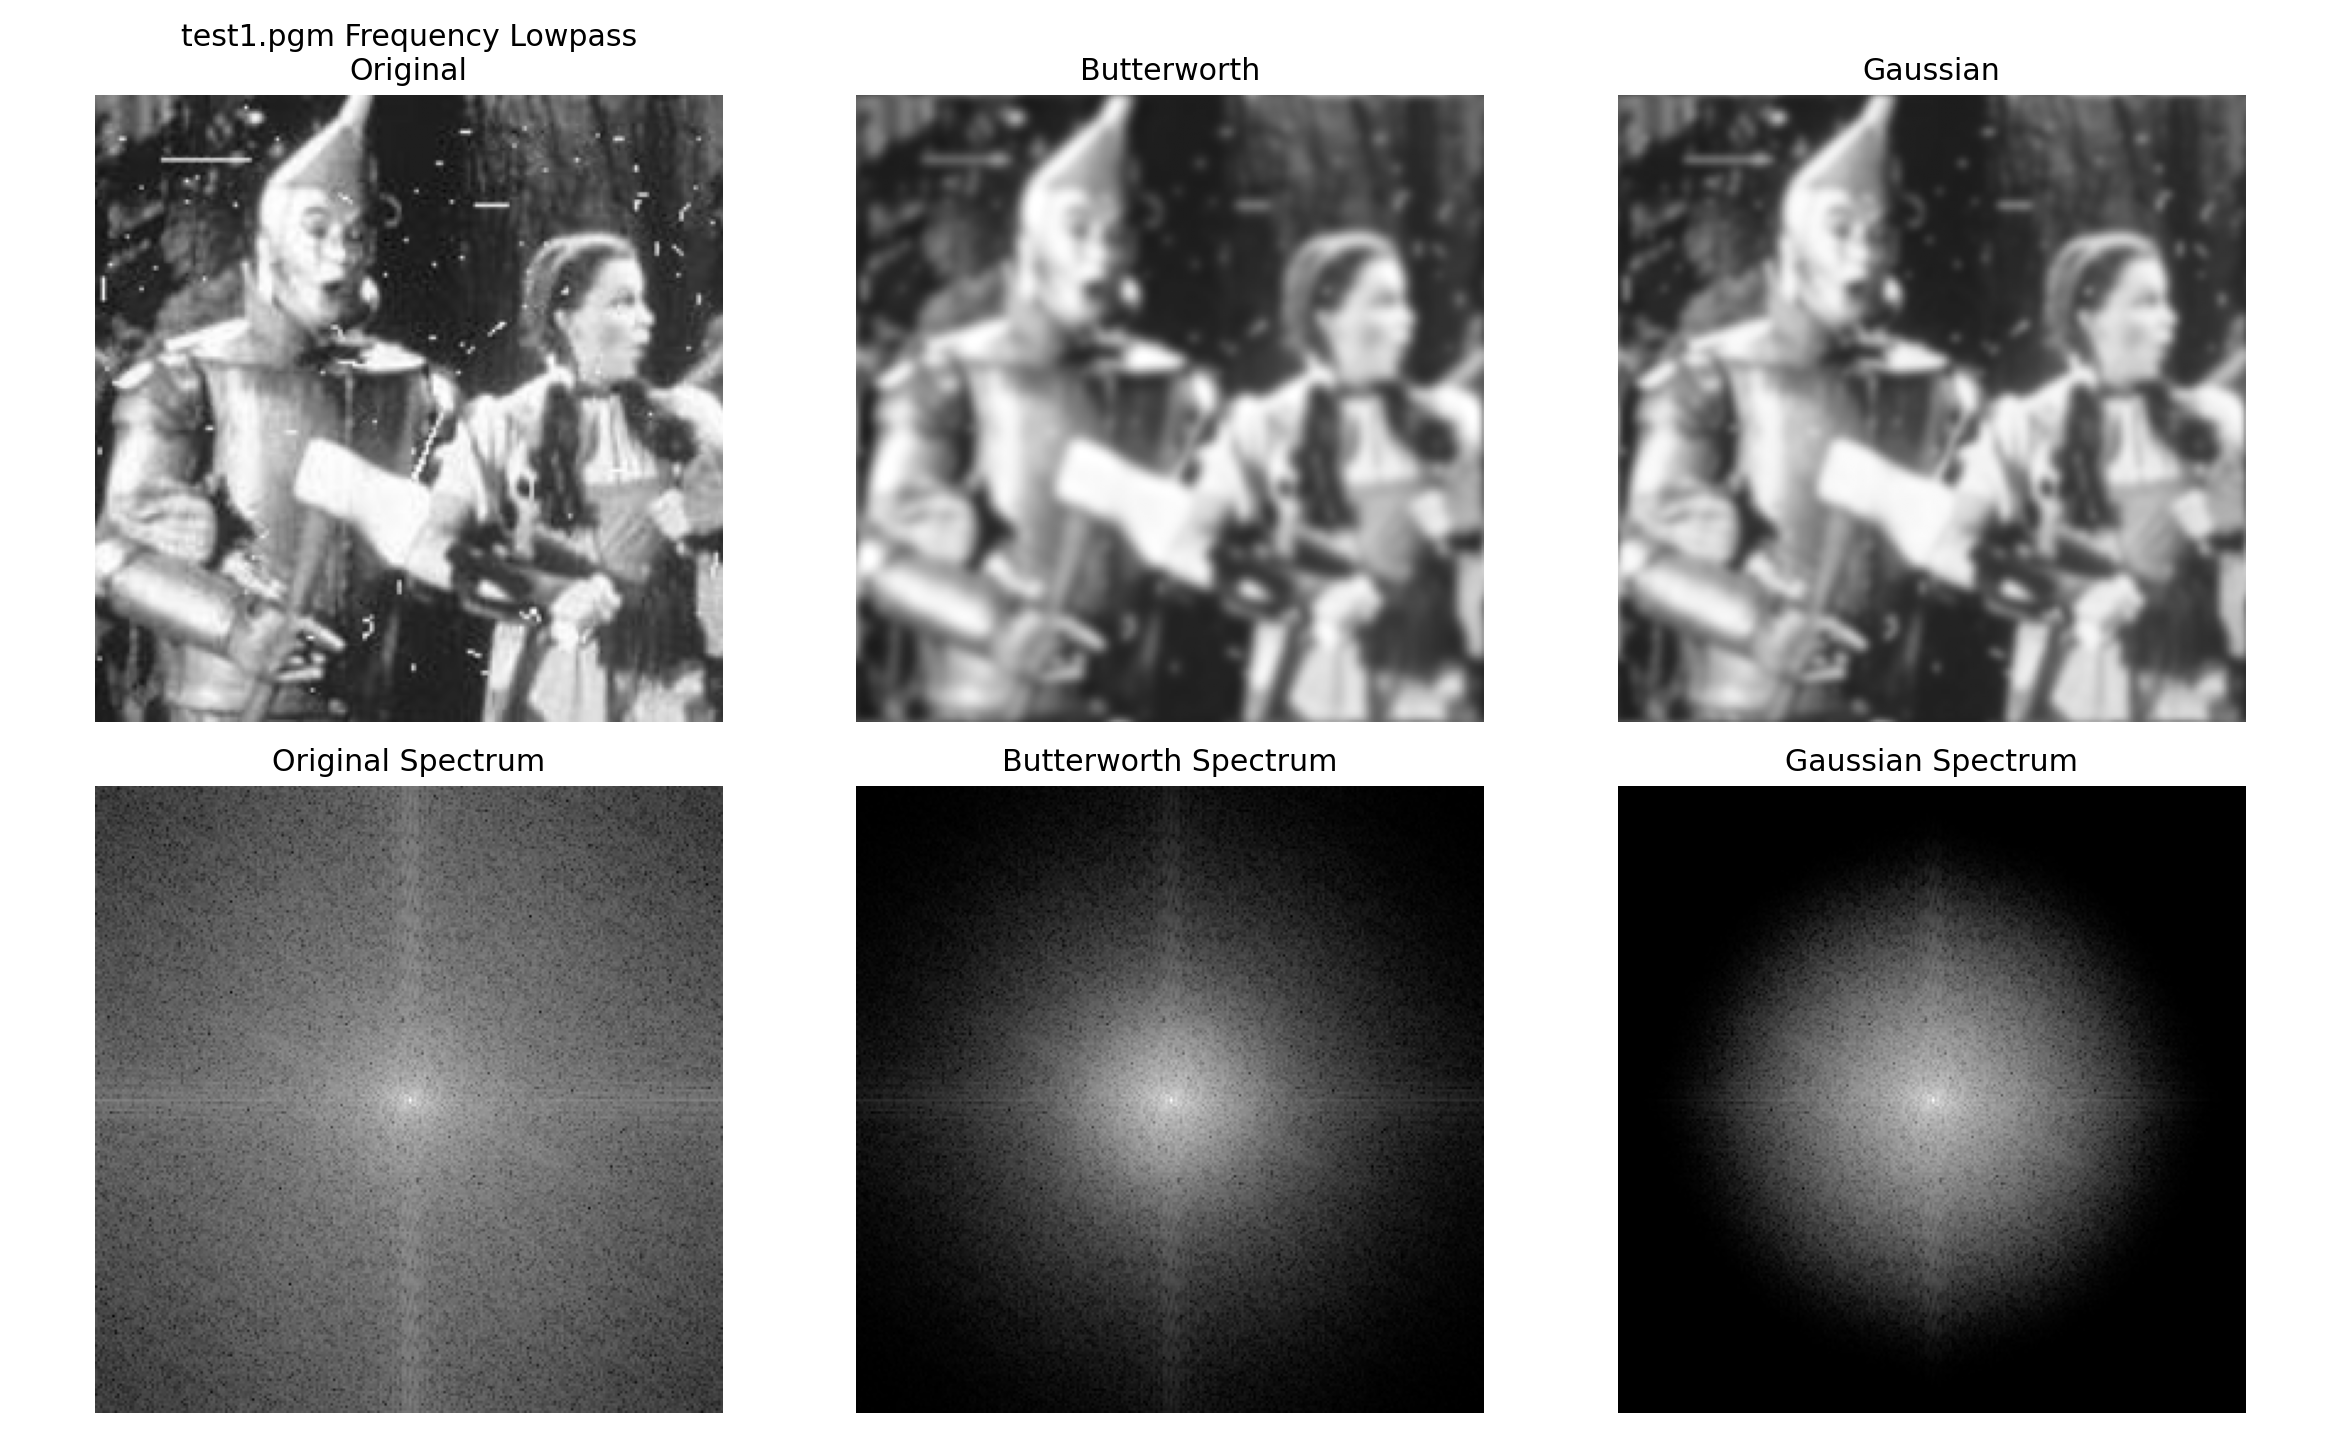
\includegraphics[width=\linewidth]{test1_freq_lowpass_overview.png}
    \caption{\texttt{test1.pgm}}
  \end{subfigure}
  \begin{subfigure}{0.49\textwidth}
    \centering
    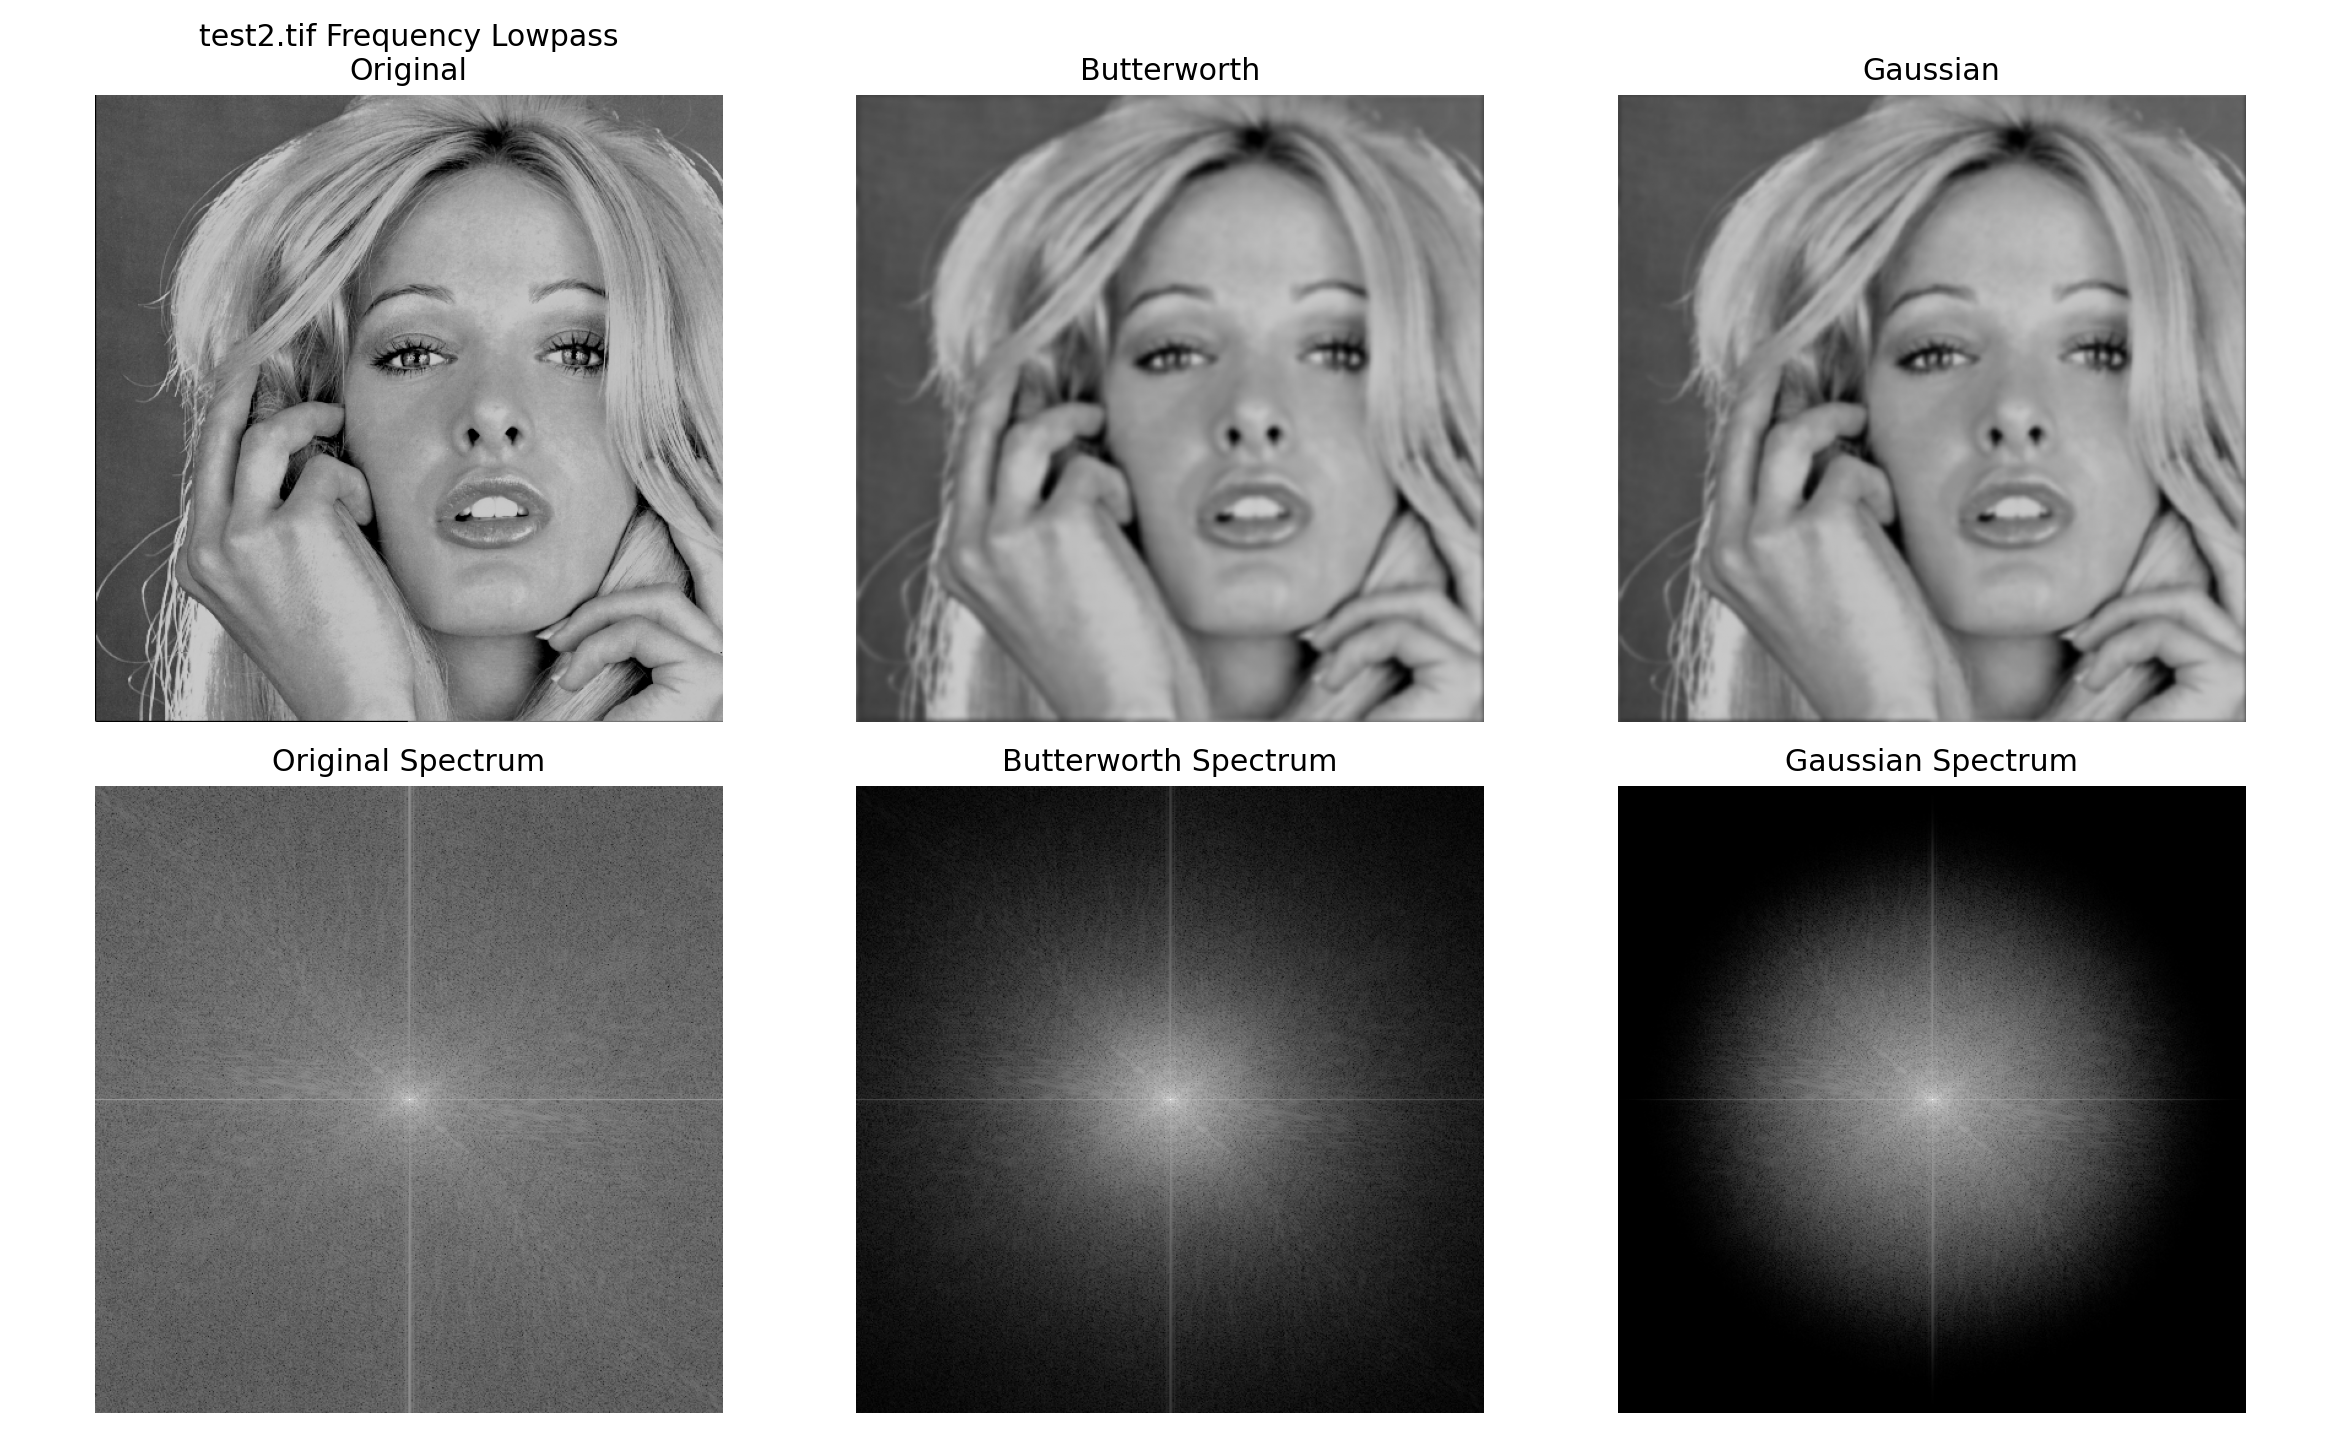
\includegraphics[width=\linewidth]{test2_freq_lowpass_overview.png}
    \caption{\texttt{test2.tif}}
  \end{subfigure}
  \caption{频域低通滤波结果总览}
\end{figure}

\begin{table}[H]
\centering
\caption{频域低通指标}
\begin{tabular}{lccccc}
\toprule
图像 & 方法 & 半径 $D_0$ & 功率谱比 & gradient\_mean & laplacian\_var \\
\midrule
test1.pgm & Butterworth LP & 25 & 0.9743 & 64.682 & 23.145 \\
test1.pgm & Gaussian LP & 25 & 0.9687 & 65.284 & 32.975 \\
test2.tif & Butterworth LP & 50 & 0.9885 & 28.643 & 8.187 \\
test2.tif & Gaussian LP & 50 & 0.9870 & 29.188 & 12.042 \\
\bottomrule
\end{tabular}
\end{table}

从结果可见，两种低通滤波器都明显降低了图像的高频成分，图像变得更平滑。Butterworth 低通在截止区域更陡，平滑作用更强；Gaussian 低通的频域响应更柔和，输出图像更自然，不易产生振铃伪影。

\subsection{任务2：频域高通滤波}
\begin{figure}[H]
  \centering
  \begin{subfigure}{0.49\textwidth}
    \centering
    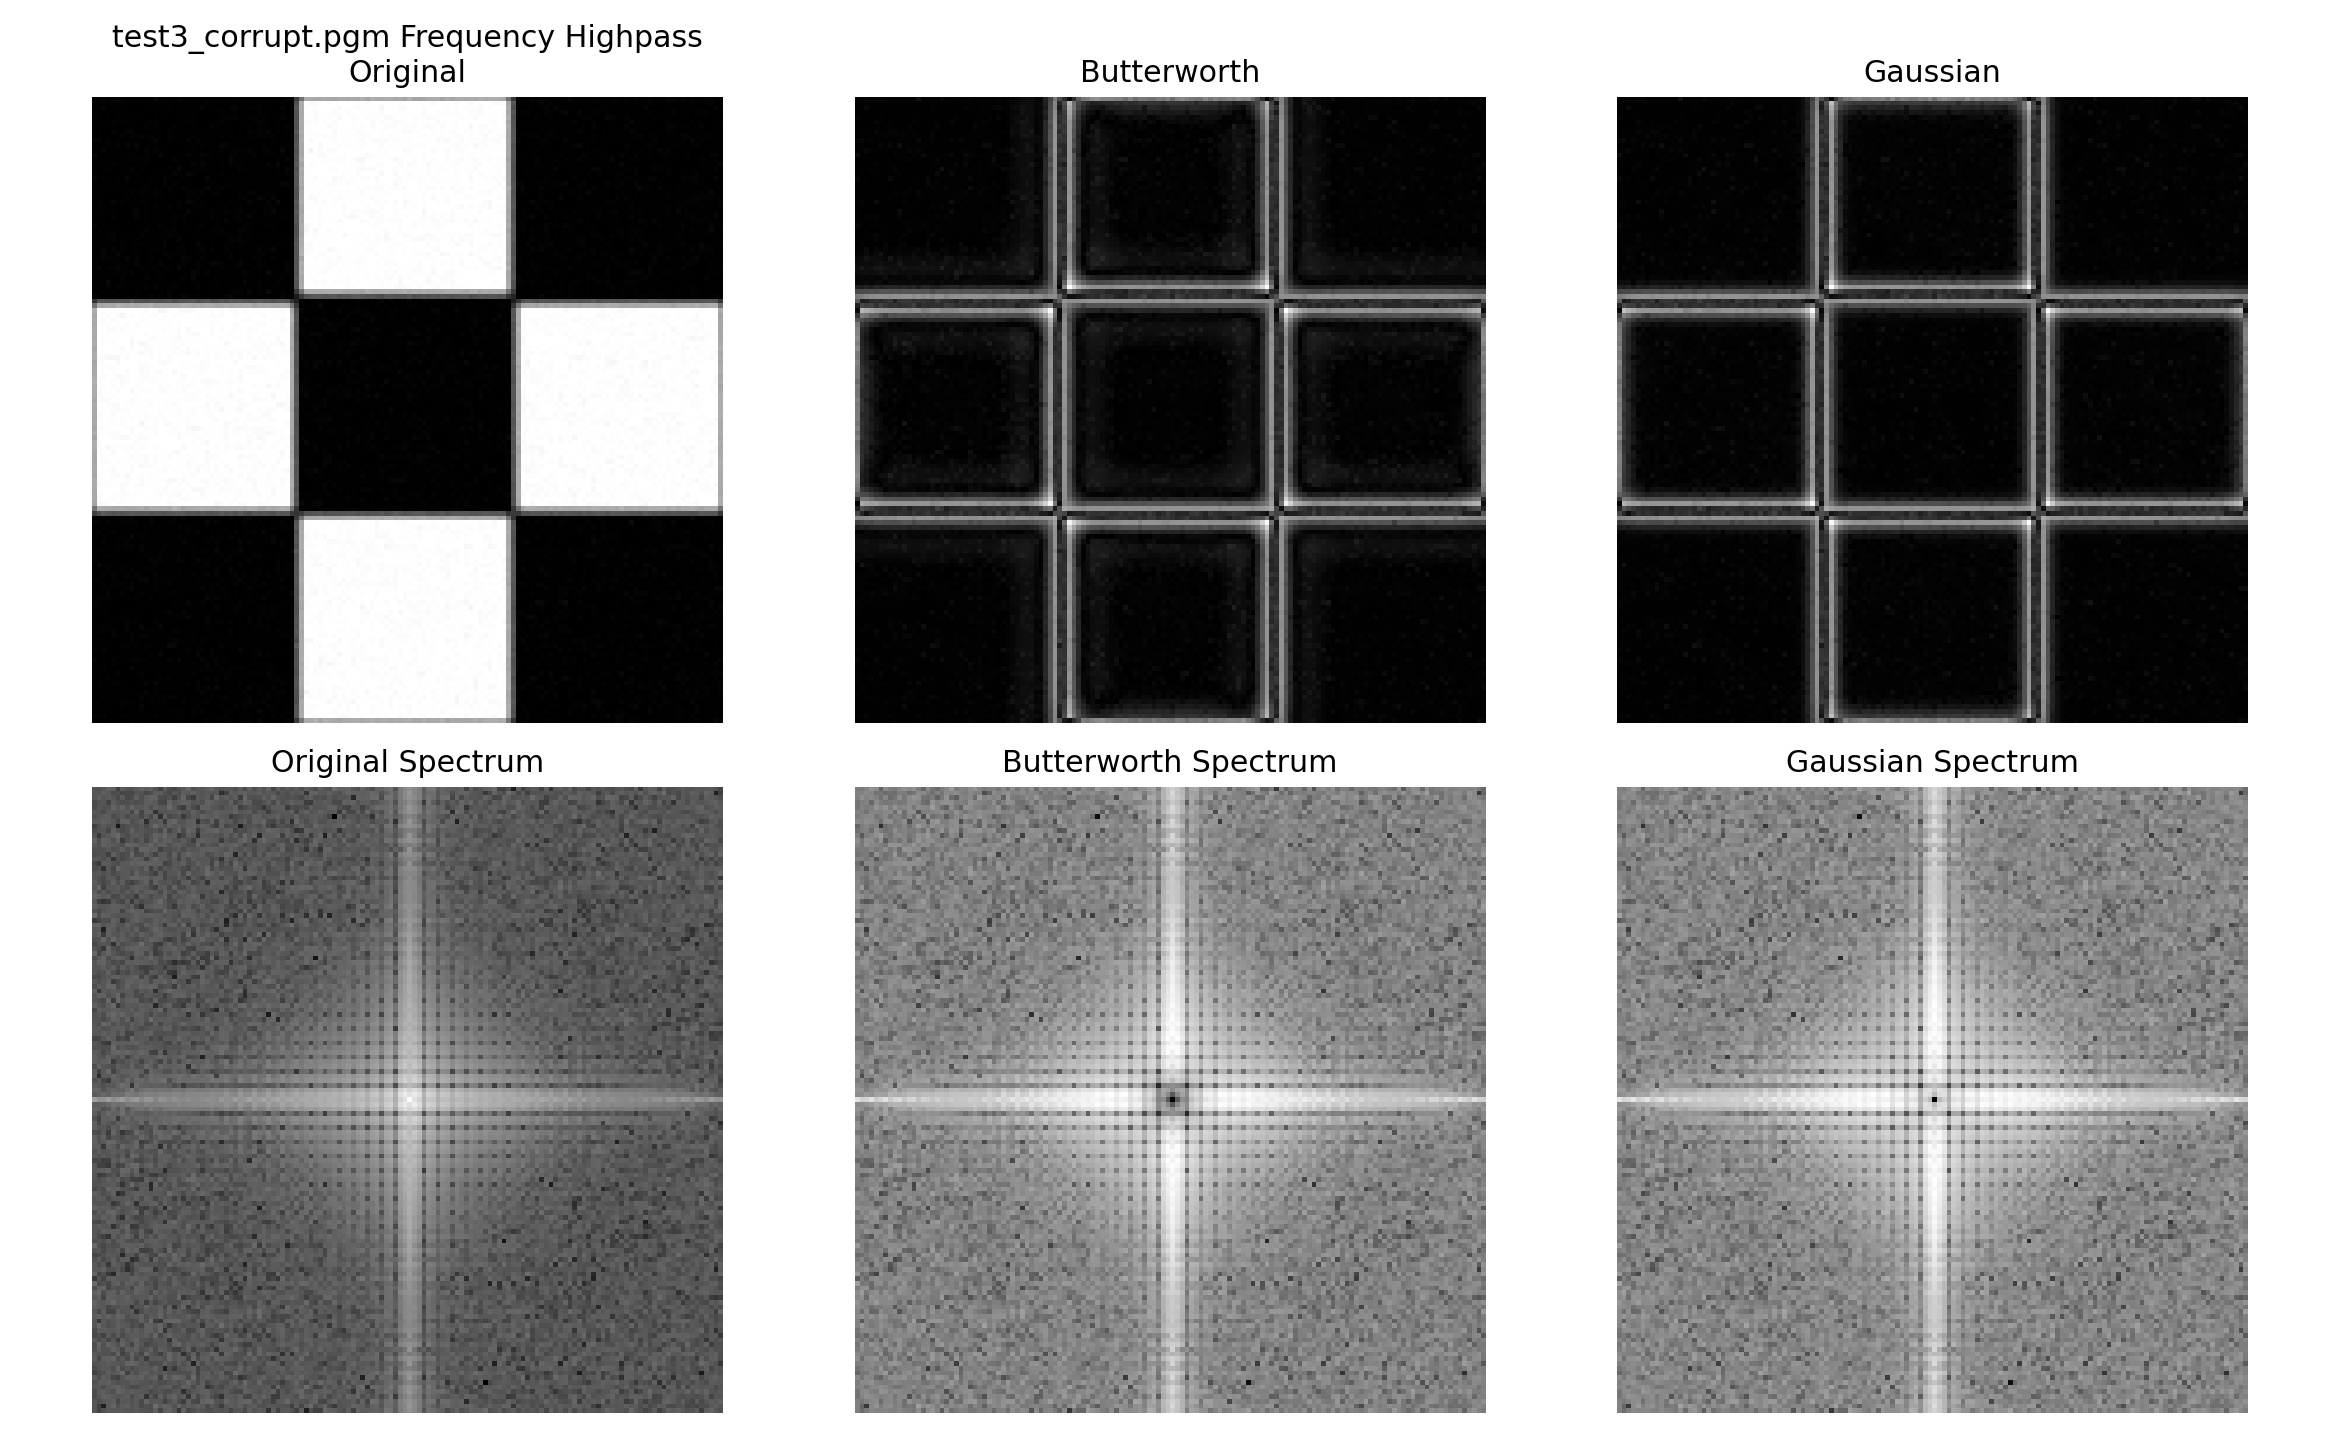
\includegraphics[width=\linewidth]{test3_corrupt_freq_highpass_overview.png}
    \caption{\texttt{test3\_corrupt.pgm}}
  \end{subfigure}
  \begin{subfigure}{0.49\textwidth}
    \centering
    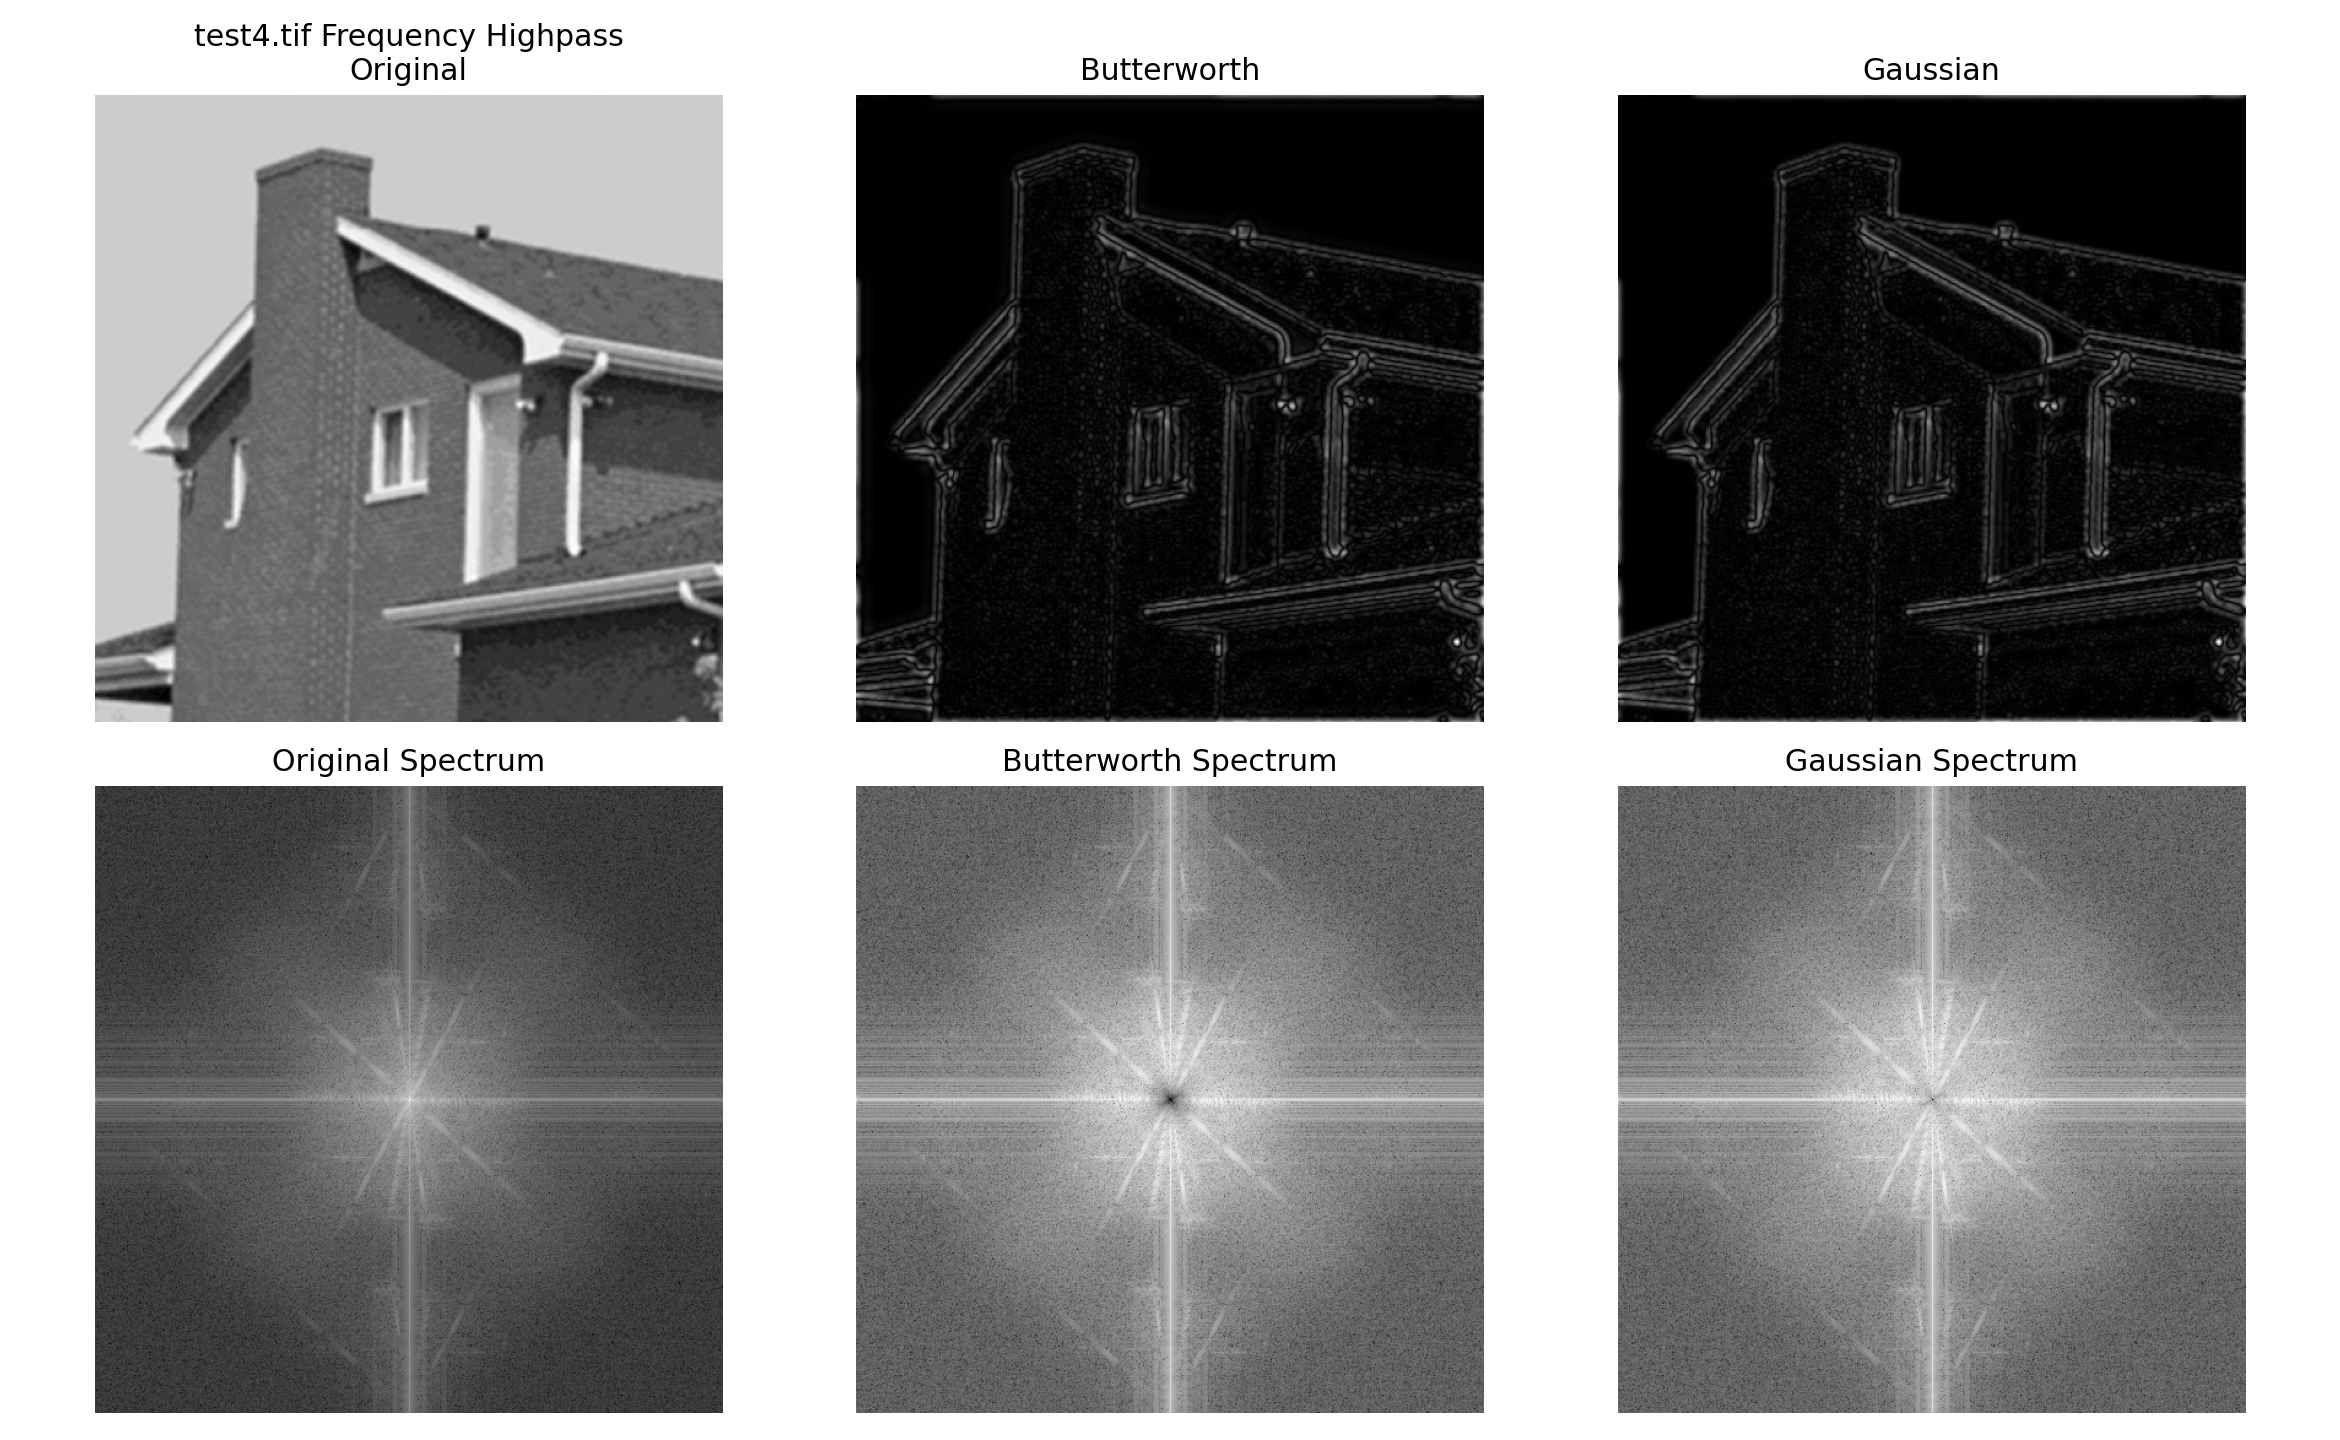
\includegraphics[width=\linewidth]{test4_freq_highpass_overview.png}
    \caption{\texttt{test4.tif}}
  \end{subfigure}
  \caption{频域高通滤波结果总览}
\end{figure}

\begin{table}[H]
\centering
\caption{频域高通指标}
\begin{tabular}{lccccc}
\toprule
图像 & 方法 & 半径 $D_0$ & 功率谱比 & gradient\_mean & laplacian\_var \\
\midrule
test3\_corrupt.pgm & Butterworth HP & 10 & 0.0183 & 98.364 & 2659.346 \\
test3\_corrupt.pgm & Gaussian HP & 10 & 0.0148 & 91.901 & 2768.905 \\
test4.tif & Butterworth HP & 30 & 0.0051 & 45.280 & 251.381 \\
test4.tif & Gaussian HP & 30 & 0.0041 & 45.262 & 279.864 \\
\bottomrule
\end{tabular}
\end{table}

高通滤波结果说明，高频能量虽然占总能量比例较小，但对边缘结构影响很大。Butterworth 高频增强通常更“硬”，轮廓更明显；Gaussian 高频增强过渡更平滑，边缘更自然。

\subsection{任务3：其他高通滤波器}
\begin{figure}[H]
  \centering
  \begin{subfigure}{0.49\textwidth}
    \centering
    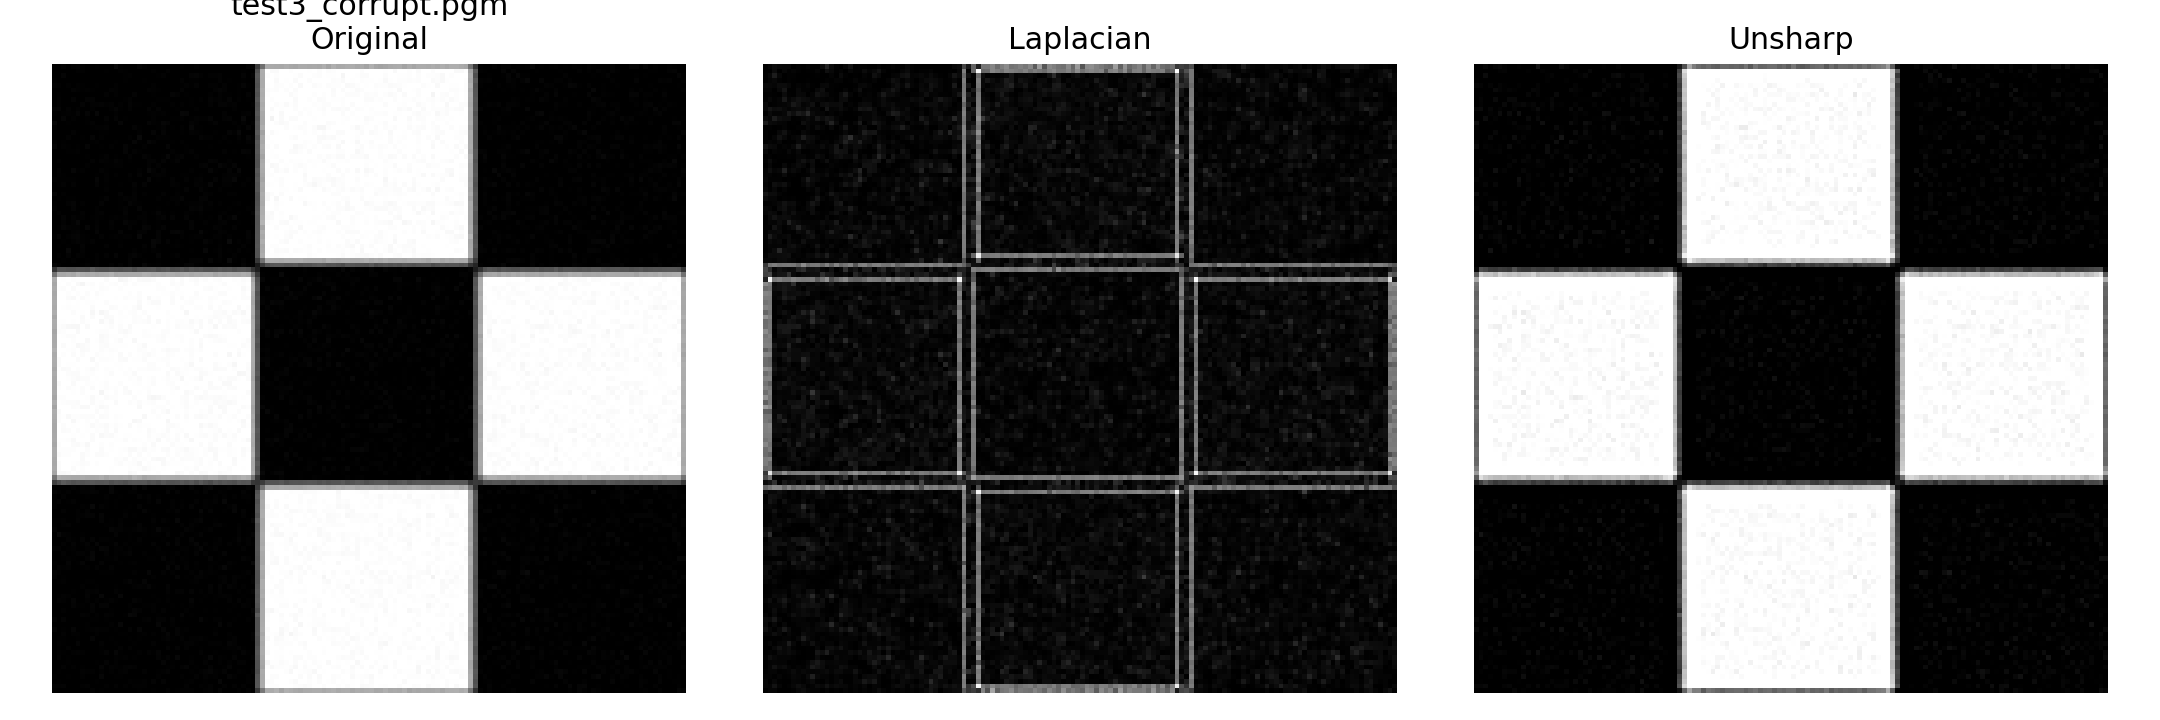
\includegraphics[width=\linewidth]{test3_corrupt_other_highpass_overview.png}
    \caption{\texttt{test3\_corrupt.pgm}}
  \end{subfigure}
  \begin{subfigure}{0.49\textwidth}
    \centering
    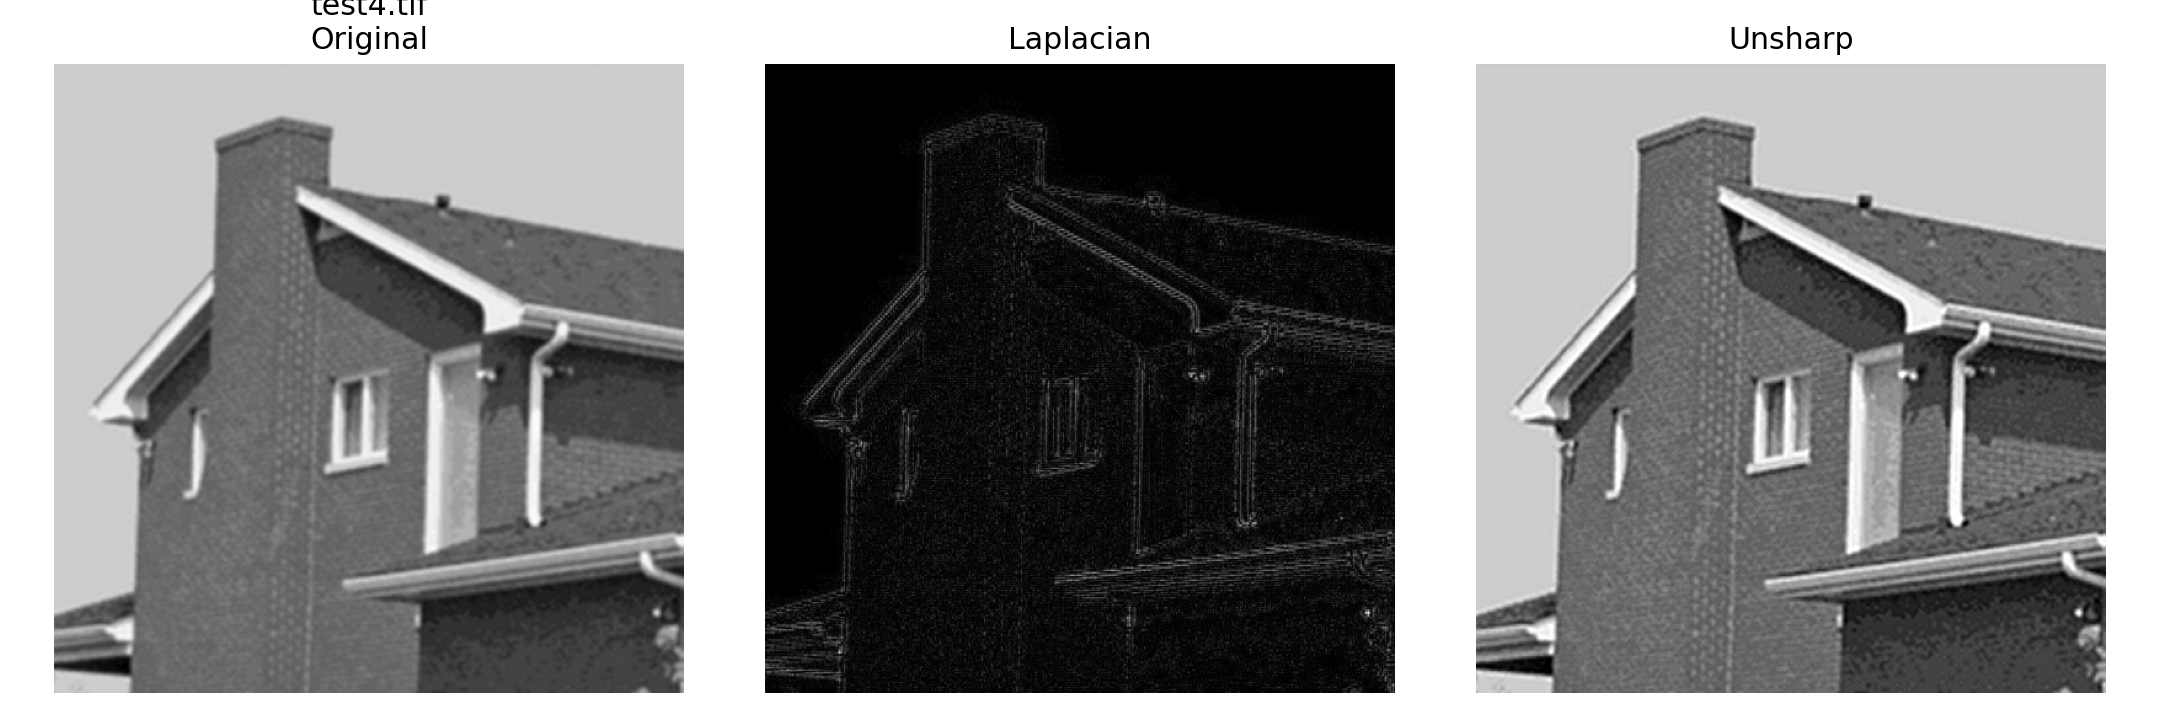
\includegraphics[width=\linewidth]{test4_other_highpass_overview.png}
    \caption{\texttt{test4.tif}}
  \end{subfigure}
  \caption{Laplacian 与 Unsharp 结果对比}
\end{figure}

\begin{table}[H]
\centering
\caption{其他高通滤波器指标}
\begin{tabular}{lcccc}
\toprule
图像 & 方法 & mean & gradient\_mean & laplacian\_var \\
\midrule
test3\_corrupt.pgm & Laplacian & 16.879 & 89.258 & 5484.053 \\
test3\_corrupt.pgm & Unsharp & 108.813 & 81.386 & 1231.188 \\
test4.tif & Laplacian & 11.599 & 43.389 & 1329.777 \\
test4.tif & Unsharp & 136.515 & 48.464 & 113.030 \\
\bottomrule
\end{tabular}
\end{table}

Laplacian 对细微灰度变化非常敏感，因此轮廓增强明显，但也会同时强化噪声。Unsharp 更适合锐化增强，因为它保留了原图外观并强化了局部细节，不像 Laplacian 那样直接输出以边缘为主的图像。

\subsection{频域与空域滤波关系讨论}
理论上，空域卷积等价于频域乘法。若频域滤波器 $H(u,v)$ 恰好是某个空域冲激响应 $h(x,y)$ 的傅里叶变换，则两种滤波方式是等效的。然而在实际离散图像处理中，两者通常不会完全一致，主要原因如下：
\begin{enumerate}
  \item 图像尺寸有限，频谱本身是离散采样结果；
  \item 边界处理方式不同，如零填充、镜像扩展等会影响结果；
  \item 空域滤波器通常采用有限模板，而频域滤波器常从连续理想函数出发再做离散采样；
  \item 参数之间往往不能严格一一对应。
\end{enumerate}
因此，空域低通/高通与频域低通/高通在趋势上是一致的，但具体数值和细节表现未必完全相同。频域滤波可以看作从整体频率结构角度进行调制，而空域滤波更像是在局部邻域内直接操作像素。

\subsection{优缺点总结}
\begin{table}[H]
\centering
\caption{各方法优缺点总结}
\begin{tabular}{p{3cm}p{5cm}p{5cm}}
\toprule
方法 & 优点 & 缺点 \\
\midrule
Butterworth 低通 & 截止更明显，平滑作用较强 & 过渡不如 Gaussian 平滑，可能有轻微振铃 \\
Gaussian 低通 & 响应平滑，结果自然 & 高频抑制相对更柔和 \\
Butterworth 高频 & 边缘增强更直接、更明显 & 对噪声更敏感 \\
Gaussian 高频 & 过渡自然，伪影较少 & 边缘增强相对更温和 \\
Laplacian & 对轮廓和细节很敏感 & 噪声容易被同步放大 \\
Unsharp & 适合锐化增强，保持原图外观 & 不是纯边缘图，参数不当会过锐 \\
\bottomrule
\end{tabular}
\end{table}

\section{结论}
\begin{enumerate}
  \item 频域低通滤波能够有效削弱高频成分，实现图像平滑；其中 Gaussian 低通结果更自然，Butterworth 低通更强调截止效果。
  \item 频域高通滤波能够突出边缘和细节；Butterworth 高频更强烈，Gaussian 高频更平滑。
  \item Laplacian 更适合提取强边缘信息，Unsharp 更适合增强原图细节与清晰度。
  \item 空域滤波与频域滤波理论上等效，但在实际数字图像处理中通常只在趋势上对应，不会完全一致。
\end{enumerate}

\section*{AI Report}
本次实验在题目理解、代码实现、参数整理、结果统计和报告撰写过程中使用了 AI 辅助。AI 主要参与了以下工作：根据题目要求生成频域滤波与空间域高通处理代码；自动输出结果图、频谱图和指标表；辅助整理功率谱比、空域与频域关系等理论解释；辅助生成实验报告初稿。最终实验结果、参数选择和报告内容均经过人工检查、确认和修改。

\section*{附：编译与使用说明}
\begin{itemize}
  \item 建议在 Overleaf 中选择 \textbf{XeLaTeX} 编译器。
  \item 上传本文件 \texttt{report\_hw5\_overleaf.tex} 与 \texttt{outputs/} 整个文件夹即可。
  \item 本文图片均直接引用 \texttt{outputs/task1\_freq\_lowpass}、\texttt{outputs/task2\_freq\_highpass} 和 \texttt{outputs/task3\_other\_highpass} 中的结果。
\end{itemize}

\end{document}
